%************************************************
%\chapter{A model for distributed web-based human- and machine-driven computation}
\chapter{The Model}
\label{cap:model}
%************************************************


% il mio sistema ha una logica di associazione del task
% quale task a chi e con quale codice


% Cubrick METADATA MODEL!!!!!!!!
% definisco l'architettura, chi sono gli attori
% definisco il modello degli attori (task, utente, uTask, client) e come sono relazionati
% ES
% relazione n->n task client
% Il task può essere svolto da codici diversi in funzione del client


% in questo capitolo definiamo il modello del nostro sisstema diviso in
% modello architetturale, modello dei dati e modello di esecuzione
% infine presentiamo la logica di pluggabilità delle strategie (quelle
% di default e quelle custom)











% TODO: cambiare il nome: no system model!
\newcommand{\model}{\emph{architectural model}}
In this chapter, we define the \model for our system and the reference
infrastructure supporting this model.
The \model is the data model on which the single components of the system are build upon.
It describes the components that interact each other during the task lifecycle and
embodies also the requirements and the features of the system as expressed in
the \hyperref[intro]{introduction}.\\



Concerning the data model we have subdivided it in 3 parts, this subdivion is made to
better distinguish each of the 3 main steps used in every distribution system in order
to create, distribute and process the data. \autoref{fig:model} gives an overview of
the \model that is composed by:
% model subdivision
\begin{description}
	\item[The {\hyperref[sec:model:data]{data model}}:] describes
	the data structure used to create this system.

	\item[The {\hyperref[sec:model:architecture]{architectural model}}:] describes
	the reference architecture of the sytem.
	
	\item[The {\hyperref[sec:model:execution]{execution model}}:] focuses
	on the execution model of the task.

	\item[{\hyperref[sec:model:strategies]{Pluggable strategies}}:] here
	are provide some example of strategy that can be plugged to the system.
\end{description}



% Sezioni
\section{Data model}
\label{sec:model:data}
% Data Model
data model


% task con custom proiperties in modo da configurare i runtime

\section{Architectural model}
\label{sec:model:architecture}
\begin{figure}[htb]
	\centering
	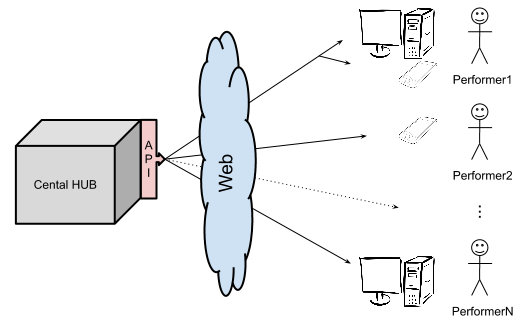
\includegraphics[width=0.75\columnwidth]{Architecture}
	\caption{Reference architecture.}
	\label{fig:architecture}
\end{figure}
% TODO nell'immagine metto anche un dispositivo mobile e un utente con 2 device

During the Design Process we faced the problem of finding a suitable Architectural
Model able to support all the requirements, in terms of flexibility and pluggability,
raised during the Process Design. In our model we use as a reference architecture
the one depicted in \autoref{fig:architecture}. Here we have a central hub
in charge of distributing the Tasks to the nodes\footnote{We refer to nodes
because we want to enclose both humans and devices.} and an abstraction layer.

The \emph{Central Hub} is used to manage all the data exchange between to the
nodes and the hub itself, orchestrating all the communication flow.

The \emph{Abstraction Layer} is used to normalize the differences between the
nodes, creating a coherent representation of nodes.\\




As described in \ref{design:work}, our framework has multiple configuration
points used to customize the Task behavior. As described in \vref{data:task},
for each Task we identified seven configuration points:
\begin{description}
	\item[\utask{} planning strategy:] defines how many \utask{} to create for
	each Task and associate the right portion of Objects to each of them.
	\item[\utask{} implementation strategy:] defines the logic behind the choice
	of a \utask{} implementation sent to a user.
	\item[Performer assignment strategy:] in charge of choosing the users who
	are suitable to execute a certain Task.
	\item[Task Planning strategy:] orchestrates the invocation of the \utask{}
	planning strategy, the \utask{} implementation strategy and the Performer
	assignment strategy.
	\item[Task Control strategy:] defines a controller for the Task, able to
	check the status, and if needed, perform corrective actions.
	\item[Aggregation function:] is in charge of joining the results obtained
	from the \utask{}s execution and create a Task output.
	\item[Emission policy:] is used to rule notifications sent to the Subscribers.
\end{description}
All these configuration points are described in \ref{sec:model:strategies}.

\section{Execution model}
\label{sec:model:execution}
% Execution model
Execution model

\section{Pluggable strategies assignment}
\label{sec:model:strategies}
%% Pluggable+Strategies

As pointed out during the Process Design and briefly introduced in the 
Architectural Model, our framework must be able to handle custom strategies.
These strategies (see \ref{sec:model:architecture}) are used to grant that
our model is flexible enough to support all the application archetypes
defined in \autoref{tab:matrix}.

This section explains the purposes of each strategy and what are the
main properties for each strategy.


\subsection{\utask{} Planning strategy}
The \utask{} Planning strategy is a pluggable logic devoted to the creation, or
deletion, of \utask{}. Eventually this strategy must, during the creation
time of a \utask{}, bind a corresponding set of Task Objects to the \utask{}.
This binding produce a set of \utask{} with the corresponding Task Objects. A
Task planning strategy is defined by:
\begin{itemize}
    \item A set of \textbf{Constraints} that rules the execution.

    \item A \textbf{Planning policy} that can be defined at:
        \begin{description}
            \item[Design time:] the assignment is made at design time during the
            creation phase. After the planning is done it can be modified only

            \item[Dynamic:] the planning is done at least once, using a provided
            set of input \emph{Object}s. The planning can be further invoked due
            to:
            \begin{itemize}
                \item \emph{Variations} in the state of the Task. i.e. an object
                can be reassigned to another \utask{}.

                \item \emph{Addition} of new \emph{Object}s through the API.
            \end{itemize}
            Note that the addition of new \utask{} can be performed using the
            API but usually do not involve the invocation of a \utask{} planning
            strategy.
        \end{description}
\end{itemize}



\subsection{Performer Assignment strategy}
The Performer assignment strategy is a pluggable logic devoted to the assignment
\emph{Performers} to \utask{}. Once we have a set of \utask{} we can assign to
them the suitable Performers. The Performers are chosen according to some
criteria like their skills or the place they live. A Performer assignment
strategy is composed by:
\begin{itemize}
    \item A \textbf{set of Constraints} defined on top user-specific statistics
	(e.g. do not assign more than 1 \utask{} per hour).

    \item A \textbf{list of routes} that, by matching the description of a
    \emph{Performer}, decide if a \utask{} can be assigned to that \emph{Performer}.

    \item An \textbf{Invitation Strategy}, which defines how performers should be 
    invited to execute the task.

    \item An \textbf{Assignment policy} that can be:
        \begin{description}
            \item[static:] the assignment can be performed both at design time and
            runtime, but it must be explicitly called by a control rule.
            \item[dynamic:] the assignment is performed at least once and can be
            invoked multiple times later according to \emph{Variables} that can
            change over time.
        \end{description}
\end{itemize}



\subsection{\utask{} Implementation strategy}
\utask{} Implementation strategy is a pluggable logic in charge of selecting a
suitable \utask{} implementation for an \emph{Execution}. This strategy is invoked
before the execution of a Task on a device. Based on the Performer preferences
or on the device characteristics a suitable \utask{} implementation is routed to
the user.


\subsection{Task Planning strategy}
The Task Planning strategy embodies the functionalities of a \utask{} Planning
strategy and Performer Assignment strategy, deciding the logic by which the
two strategies should be invoked. This strategy can be used to manage the
re-planning of the \utask{}s or to call the Performer Assignment strategy. The
invocation of this strategy is controlled by the Task Control strategy that can
call this strategy upon changes in the Task status.




\subsection{Task control strategy}
The Task control strategy is a pluggable logic devoted to verifying the status of
a Task, possibly against the assigned constraints. This logic can be executed:
\begin{itemize}
    \item \textbf{Once} when the Task ends. For instance when all the \utask{}s
    are executed to re-plan the execution.

    \item According to a \textbf{temporal schedule} (i.e. every $x$ minutes,
    once a day, at noon, etc.).

    \item Every time a \utask{} is \textbf{executed}.
\end{itemize}
\noindent Among the corrective actions available to the Task controller we have: 
\begin{itemize}
    \item The \textbf{re-planning} of the task, also with the creation of new
    \utask{}.

    \item The \textbf{re-assignment} of \utask{} to \emph{Performer}s.

    \item \textbf{Deletion} of executed \utask{}.

    \item \textbf{Change} the properties of an executed \utask{}. For instance
    we can set the results as invalid if we have spotted a cheater.

    \item \textbf{Re-execution} of the entire Task.

    \item \textbf{Halting} the Task.

    \item etc.
\end{itemize}



\subsection{Aggregation function}
An Aggregation function is a pluggable logic devoted to joining the results
obtained with the \utask{}s execution. These results are merged according to a
Task specific logic in order to produce the Task output result. An aggregation
function can be as simple as a \emph{Sum} or an \emph{Average} but can can also
be more complex. For instance we can gather the results obtained, perform
filtering operation and eventually produce an image.


\subsubsection{Emission policy}
The Emission policy controls how the \emph{Subscribers} are notified about the
status changes in a Task. This logic can be executed:
\begin{itemize}
    \item \textbf{Once} the Task ends.

    \item According to a \textbf{temporal schedule}.

    \item Every time a task is \textbf{executed}.
\end{itemize}
